\epigraph{\textit{Simplex sigillum veri (The simple is the seal of the true) \\ 
Pulchritudo splendor veritatis (Beauty is the splendor of truth) } \\ \vspace{3mm} Latin phrase } 

The theory of the renormalization group (RG) flow has been one of the most important ideas in Physics in the last century. 
The fixed points of the RG flow constitute an important class of quantum field theories, known as conformal field theories (CFT). 
A quantum field theory is a conformal field theory when the action is invariant under conformal transformations. 
The conformal invariance highly constrains the field theory and has far-reaching implications such as vanishing of 
the energy-momentum tensor. However, in some cases, a quantum process can break this symmetry and give rise 
to trace anomaly and non-zero stress tensor. The CFT can then be completely described by central charges of the 
energy-momentum tensor. These central charges determine the correlation function of the theory and also 
reorient the theory under renormalization group flow. It is known (in two dimensions) using Zamolodchikov's c-theorem \cite{Zamolodchikov:1986gt} 
that the central charge $c$ increases from the infrared (IR) to the ultraviolet (UV). 
This theorem orders a CFT and provides interpretation of the central charge as
measure of the field degrees of freedom in the theory. These degrees of freedom decrease along the renormalization
flow due to the decoupling of massive modes. The study of CFTs has also been very much pursued in recent years due to holographic 
application via the AdS/CFT correspondence. The results for the entanglement entropy obtained from CFT 
in lower dimensions agrees to the calculations using gravity. 

However, it is highly unusual for any theory to have a line 
of fixed points all along the RG flow and to be conformal under quantum interactions. 
One such special theory in Physics is $\mathcal{N}=4$ super Yang-Mills (SYM) theory in four dimensions. 
This theory is maximally supersymmetric and has sixteen supercharges. 
This virtue of fixed points is solely because of supersymmetry \footnote{A non-supersymmetric theory 
which shows this behavior of line of fixed points is XY 
model in two dimensions for $T \le T_{KT}$}. Since this is such an interesting theory, one desires to understand its 
properties non perturbatively as well. This motivation has resulted in several decades of work of realizing the 
supersymmetry on the lattice which furnishes a gauge-invariant regularization to study the theory at strong couplings. $\mathcal{N}=4$ SYM
is also special because it takes part in the AdS/CFT correspondence, the first concrete example of a 
holographic correspondence between supersymmetric gauge theory and a gravity theory on anti-deSitter (AdS)
spacetime \cite{Maldacena:1997re, Itzhaki:1998dd, Aharony:1999ti}. 
For a nice discussion on lattice gauge theory and AdS/CFT correspondence, see ~\cite{Caselle:2000tn}.

The non-perturbative features of supersymmetric Yang-Mills (SYM) is thought to play a crucial role in the beyond 
Standard model (BSM) Physics and also in M/String theory. 
The non-perturbative study of string theory is based on various matrix models. 
In general, two kinds of non-perturbative formulations of M/string theory are developed. The first is called the Matrix theory. 
The typical examples are BFSS Matrix model and the
plane wave Matrix model (PWMM) which describes a sector
of M theory with the definite light-cone momentum on flat
background and pp-wave background, respectively. There is another 
0+0-dimensional matrix model called IKKT model \cite{Ishibashi:1996xs}. 
These matrix models are dual to classical supergravity only in the large $N$ and strong coupling limit which 
is in general not analytically solvable. In the last ten years, there have been several precision numerical calculations 
which have reproduced predictions from the dual gravity providing a piece of very strong evidence about the validity of 
the holographic conjecture, which we will discuss in detail in Chapter 3. 

BFSS matrix model (like many extended supersymmetric models) has a moduli space. 
The moduli space in this theory is given by the eigenvalues of nine commuting matrices i.e $ [X_{i}, X_{j}] = 0 $ 
that transform under the SO(9) R-symmetry. The existence of these flat directions means that, at finite temperature,
the partition function is formally divergent, and it was shown that when Monte
Carlo simulations of this theory are performed, this divergence eventually causes the
simulation to break down. The second kind of approach to a non-perturbative approach to string theory/M-theory 
is via the AdS/CFT correspondence. It was first studied by Maldacena for which the pair system was 
Type IIB supergravity on AdS$_5 \times S_5$ and $\mathcal{N}$ = 4 SYM.
Using this duality, several results for the strongly coupled field theory have been reproduced by the classical 
gravity in the bulk. However, the other direction, $\emph{i.e.}$
getting some results for gravity from field theory has been less explored because of lack of calculational tools in 
the strongly coupled field theory. This thesis attempts to explore this side of duality by using lattice as a tool for 
dealing with strongly coupled field theory. 
In addition, lattice also provides a window into the finite-$N$ and coupling corrections to the leading holographic 
result only valid in $N \to \infty$ and $\lambda \gg 1$. This is shown in more detail in Figure \ref{fig:Nlam1}. 


\begin{figure}
\begin{center}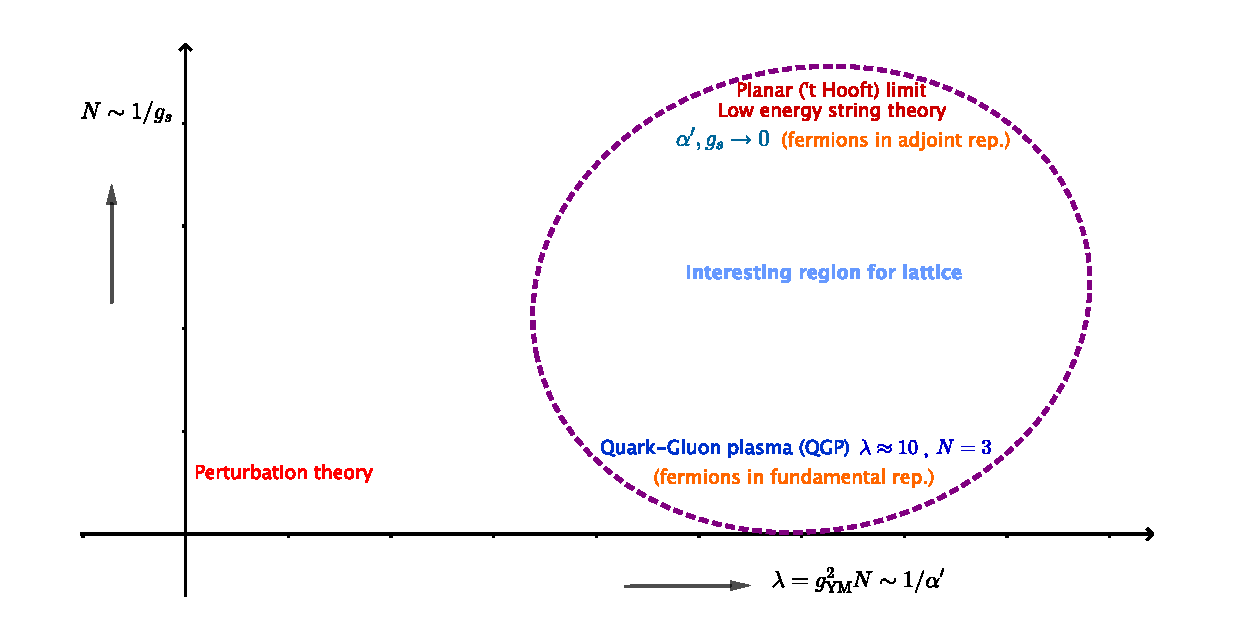
\includegraphics[width=0.85\textwidth]{./Figures/N_lam_phase.pdf}\end{center}
\caption{\label{fig:Nlam1}Different regions of supersymmetric/non-supersymmetric gauge theories in the $N-\lambda$ plane}. 
\end{figure}

\section{Supersymmetry (SUSY)}

Supersymmetry is a theoretical idea which relates half-integer (fermions) and
integer-spin (bosons). For a nice review on supersymmetry and its lattice constructions, 
see \cite{Argyres:2001eva, Seiberg:1997ax, Catterall:2009it}. 

The roots of supersymmetry were laid when Coleman and Mandula (CM) proved a theorem ~\cite{Coleman:1967ad} 
which was then supposed to be the final nail in the discussion of how the Poincare group and internal symmetries can 
be mixed together. 
They showed that under some assumptions, there was no non-trivial way of combining the two. In a way, it meant that 
there cannot be any manner in which the fermions can be brought on the same footing as bosons. But, then, physics 
thrives on crisis and exceptions. A few years later, Haag, Lopuszanski and Sohnius ~\cite{Haag:1974qh} showed that the 
showed that if some of the assumptions in the Coleman-Mandula theorem are relaxed then it is possible to mix these symmetries. 
This implied the use of graded Lie algebra instead of the normal Lie algebra which was used in the argument by CM.  


\subsection{Extension of the space-time symmetry group} 
The Poincare group is composed of transformations of the form, 
\begin{equation}
x^{\mu} \rightarrow x^{\prime \mu} = \Lambda^{\mu}_{\hspace{1mm} \nu} x^{\nu} + a^{\mu}
\end{equation}

We talk about Lorentz transformations if in the above transformation we do not have the $ a^{\mu}$ part. Hence, it is pretty obvious to
imagine Poincare transformations as a direct product between Lorentz transformations and group of 4-translations. 
In fact, it is not a direct but semi-direct product of two. 
The Poincare algebra is given by :
 
 \begin{equation}
 M^{\mu\nu} , M^{\rho\sigma}] = i \left (M^{\mu\sigma} \eta^{\nu\rho} + M^{\nu\rho} \eta^{\mu\sigma} - M^{\mu\rho} \eta^{\nu\sigma} - M^{\nu\sigma} \eta^{\mu\rho} \right)
 \end{equation}
 
 \begin{equation}
[P^{\mu}, P^{\nu}] = 0
 \end{equation}
 
\begin{equation}
[M^{\mu\nu}, P^{\sigma}] = i \left(P^{\mu}\eta^{\nu\sigma} - P^{\nu}\eta^{\mu\sigma}\right)
\end{equation}
here $\textbf{M}$ is the anti-symmetric generators of the Lorentz group and $ \textbf{P}$ are the translation generators. 

The CM theorem clearly meant that there was no non-trivial way of mixing particles with integer and half-integer spin. 
Wess and Zumino discovered field theoretic models with this extended symmetry (called 'supersymmetry') 
which connects Bose and Fermi fields and are generated by charge transforming like spinors under Lorentz group 
(supercharges). These supercharges give rise to a new system of commutation and anti-commutation relations, 
which is not precisely a Lie algebra but a graded algebra. This has a $ \mathcal{Z}_{2}$ grading. 
The Poincar\'{e} generators $ P^\mu$ and $M^{\mu\nu}$ are bosonic generators. In supersymmetry, we add fermionic generators $Q_{\alpha}^{L}$, $\overline{Q_{\beta}^{M}}$, where
$L, M = 1,2, \cdots \mathcal{N}$. The $\mathcal{N} = 1 $ case is simple supersymmetry and $\mathcal{N}  > 1$ is extended supersymmetry. 
The complex spinorial generators follow the following algebra, 

\begin{equation} 
\{Q_{\alpha}^{L}, Q_{\beta}^{M}\} = \epsilon_{\alpha\beta} Z^{LM}
\end{equation} 

\begin{equation} 
 [P,Q] = 0
 \end{equation} 

\begin{equation} 
[Q_{\alpha}^{L}, M_{\mu\nu}]  = \frac{1}{2} (\sigma_{\mu\nu})_{\alpha} \hspace{1mm} ^ {\beta} Q_{\beta}^{L} 
 \end{equation} 

\begin{equation} 
 \{Q_{\alpha}^{L}, \overline{Q_{\beta}^{M}}\} = \delta^{LM} \sigma^{\mu}_{\alpha\beta} P_{\mu}
  \end{equation} 

 The last one is the most interesting of these four. It roughly means that the supersymmetric generators are
 the square root of the four-momentum. It also means that combining two supersymmetric transformations 
 (one of each helicity) corresponds to space-time translation. Also, in our discussion, we neglect any central 
 charges denoted by Z in the first equation. That then reduces to,  
\[ \{Q_{\alpha}^{L}, Q_{\beta}^{M}\} = 0 \]  
This commutation relation should be enough to dissuade one from attempting to put supersymmetry on the lattice since 
infinitesimal translations don't exist on the lattice and supersymmetry is broken at the classical level. If supersymmetry is 
not consistent with lattice discretization, then one immediately asks - why do we really want to study lattice supersymmetry? 

Supersymmetry is interesting because it is a mathematically consistent and elegant theory. It is worth investigating because
of the relation between SYM theories and string theory and quantum gravity. 
Most of the features of SYM theories are at strong coupling, where we have only a handful of methods in general. 
In order to have a valid non-perturbative definition from first principles, it would be desirable to go back to the highly 
successful tool of lattice gauge theory which has produced amazing results in QCD. 
However, supersymmetry is very different from QCD and has a much richer structure and field content. 
One can immediately see this from supersymmetric algebra, which is very constrained. 
Once we fix the maximum helicity (which for theories without gravity is one, and with gravity is two), 
there are only a few possibilities for the number of supercharges (or supersymmetries) that can exist. In case of no gravity, 
the maximal number of supercharges is 
16 and for supergravity theories, it is 32. If the SYM theory possesses sixteen supercharges, 
we often refer to it as ~`maximally supersymmetric'.
The restriction on the maximal spin comes from the idea that the theory should be renormalizable.
Any supersymmetric theory is often labeled with $\mathcal{N}$, $\mathcal{Q}$, $d$  which stands for the 
number of copies of supercharges, number of supercharges, and dimension. 
For ex: $\mathcal{N}=4$ SYM theory in $d=4$ has $\mathcal{Q}=16$ (sixteen supercharges, maximal).
This theory is obtained by dimensional reduction of the ten-dimensional $\mathcal{N}=1$ SYM theory. 

A good way of deciding which higher-dimensional theory to start from is to count the number of spinor components.  
In ten dimensions, a spinor has $2^{[d/2]} = 32$ complex components which are reduced to 16 after imposing the 
Majorana-Weyl condition consecutively in that order (which can only be done where d mod $8 = 2$). 
Therefore, $\mathcal{N}=1$ SYM in ten dimensions has 16 real components. 
A Majorana spinor in four dimensions has 4 components. To obtain
$\mathcal{N}=4$ SYM in four dimensions (which has 16 real components) 
one starts with $\mathcal{N}=1$ SYM in ten dimensions just like we mentioned before. 

$\mathcal{N}=1$ SYM in four dimensions similarly has $\mathcal{Q}=4$ components. 
So, in order to construct a supersymmetric theory in two dimensions with four supercharges i.e $\mathcal{N}$ = (2,2) SYM, 
one needs to start from $\mathcal{N}=1$ SYM in four dimensions. 


\subsection{R-symmetry} 

Supersymmetric theories are endowed with a special symmetry, known as R-symmetry. 
R-symmetry is the symmetry transforming different supercharges in a theory into each other. 
For extended supersymmetry (i.e. $\mathcal{N} > 1$), the R-symmetry group becomes a 
global non-abelian group. The bosonic, fermionic fields and the supercharges form a representation of the 
R-symmetry, as well as Euclidean rotation group $SO(d)_{E}$.
$\mathcal{N}=1$ SYM in four dimensions has a U(1) R
-symmetry while the while the $\mathcal{N}=1$
SYM in ten dimensions has no R-symmetry. 
When this $\mathcal{N}=1$ SYM in ten dimensions is dimensionally reduced, 
the R-symmetry group is enlarged to $SO(10-d)$ R-symmetry. Hence, we can immediately 
see that $\mathcal{N}=4$ SYM in four dimensions has $SO(6)$ R-symmetry.
Note that this $SO(6)$ R-symmetry is exactly the same as isometries of $S^{5}$ (five-sphere) 
which takes part in the AdS/CFT correspondence. 
In our quest to understand supersymmetry on the lattice, we will now briefly review
the ideas that will be important in constructing the lattice formulation of supersymmetric theories
which preserves some subset of the supersymmetries. 



\subsection{Topological Field Theories (TFT)}

Before moving and setting the stage for the lattice formulation of the supersymmetric gauge theories, we will review
the idea of topological field theory. One of the easiest ways to construct a topological field theory is to 
take an extended space-time supersymmetric theory and \textit{twist} it. A common feature of both supersymmetric lattice
 theories and topological field theories is the presence of nilpotent scalar supercharge $\mathcal{Q}$. 
 They have actions which are $\mathcal{Q}$-exact. 
All the supersymmetric lattice theories are associated with topological field theories but the opposite is not always true. 
A topological field theory (TFT) is characterized by the following:
\vspace{3mm} 
\begin{itemize}
\item Collection of fields defined on a Riemannian manifold($\textbf{$\mathcal{M}$}$,g)
\item A nilpotent operator which is Grassmann odd
\item Physical states are in Q-cohomology class \footnote{Given the second condition above that the operator should 
be nilpotent means that it is satisfied when a particular state is annihilated by that operator (let's call it Q). Such states 
are said to be in kernel of Q. Alternatively, a state which is annihilated by Q can take a form of Q acting on something, 
such states are said to be in the image of Q. But, there may be some states which are in kernel of Q, but not in the image; 
such states are said to be in cohomology of Q.} 
\item Energy-momentum tensor is Q-exact i.e \[ T_{\mu\nu} = Q G_{\mu\nu} \]
\end{itemize}

Q is referred to as ~`BRST charge' (also BRST operator) and the Grassmann grading corresponds to the ghost number. 
In general, Q is metric independent and is the simplest situation. However, there are far more interesting cases 
where $T_{\alpha\beta}$ is a BRST commutator even when Q fails to be metric independent. There also exist cases 
where $T_{\alpha\beta}$ is not even a BRST commutator, though, it is possible even then, sometimes, to establish the
topological nature. 
Consider the change in the partition function :
\begin{equation}
Z = \int \mathcal{D} \phi e^{-S_{q}}
\end{equation}
under an infinitesimal change in the metric, we get :
\begin{align}
\delta_{g} Z&= \int \mathcal{D} \phi e^{-S_{q}} \left(-\frac{1}{2} \int_{M} d^{n} x 
\sqrt{g} \delta g^{\alpha\beta} T_{\alpha\beta}\right)\\
&=\int \mathcal{D} \phi e^{-S_{q}} \left(-\frac{1}{2} \int_{M} d^{n} x 
\sqrt{g} \delta g^{\alpha\beta} QG_{\alpha\beta}\right)\\
&=\int \mathcal{D} \phi e^{-S_{q}} Q\chi_{\alpha\beta} = \langle Q\chi_{\alpha\beta}\rangle = 0
\end{align}
where, $ \chi = - \frac{1}{2} \int_{M} d^{n}x \sqrt{g} \delta g^{\alpha\beta} G_{\alpha\beta}$. We have 
used the fact that vacuum is BRST invariant. 
This means that the partition function does not depend on the local structure of the manifold: 
Z is a topological invariant. 
Now consider the following action, 
\begin{equation}
S(\phi) = \int d^{d} x \sqrt{g} \left[g^{\mu\nu} \nabla_{\mu} \phi  \nabla_{\nu} \phi \right]
\end{equation}
where $g^{\mu\nu}$ is the Riemannian metric and $\nabla$ is the covariant derivative. We can define the energy-momentum tensor as :
\begin{equation}
T_{\mu\nu} = \frac{\delta S}{\delta g^{\mu\nu}} 
\end{equation}
and rewriting it gives, \footnote{Using the fact that Z is already independent of metric} : 
\begin{equation}
\langle T_{\mu\nu} \rangle =  \frac{1}{\mathcal{Z}}\int \mathcal{D} \phi \hspace{1mm} \left(\frac{\delta S}{\delta g^{\mu\nu}}\right) \exp\left[\frac{-S(\phi)}{\hbar}\right]  
\end{equation}
\begin{equation}
\langle T_{\mu\nu} \rangle= 0
\end{equation}
We have established that the metric variation of the partition function vanishes, and in turn that the energy-momentum tensor is zero.  
We need to examine the presence of other metric independent correlation functions in the theory. 
Let's start by considering the vacuum expectation value of an observable :

\begin{equation}
 \langle \mathcal{O} \rangle = \int \mathcal{D} \Phi e^{-S} \mathcal{O}(\Phi)
 \end{equation}
We have to derive the conditions for this execration value to be zero. 
\begin{equation}
\delta \langle \mathcal{O} \rangle = \int \mathcal{D} \Phi e^{-S} (\delta_{g} \mathcal{O} - \delta_{g} S_{q} \cdot \mathcal{O})
\end{equation}
Assume that $\mathcal{O}$ satisfies the following properties :
\begin{equation}
\delta_{g} \mathcal{O} = \{Q, T\}  \hspace{2mm} , \hspace{5mm} \{Q, \mathcal{O}\} = 0
\end{equation}
for some T, we then have :
\begin{equation}
\delta_{g}\langle \mathcal{O} \rangle = \langle \{Q, T + \chi \mathcal{O}\}\rangle = 0
\end{equation}
It is interesting to note that even though $\chi$ which depends on $V_{\alpha\beta}$ contains metric dependence, 
we have wrapped it up in form of BRST commutator and still have metric independence. TFT can be classified into
two types: 1. Schwarz type 2. Cohomological type (Witten-type). 
\begin{itemize} 
\item \textbf{Schwarz Type}: The classical action is explicitly independent of the metric. Chern-Simons theory is a 
prototype of this class of topological field theories introduced by Witten in 1980s. The metric independence implies 
that the classical stress-energy tensor of TFT vanishes. In addition, even the quantum stress-energy tensor vanishes 
because of the fact that the remaining part of quantum action has been recast as a BRST commutator.  
$ \frac{\delta S}{\delta g^{\mu\nu}} = T_{\mu\nu} = 0 $. The alternate cases where the classical action depends 
explicitly on metric is not dealt here. It is also clear from the equation below that the quantum action for Schwarz 
type theories do not enjoy the property that the quantum action is Q-exact. 
\begin{equation}
S_{q}(\phi, g) = S_{c}(\phi) + QV(\phi,g) 
\end{equation}
\item \textbf{Witten Type}: In Witten-type topological field theories, the topological invariance is more subtle. 
The lagrangian generally depends on the metric explicitly, but one shows that the expectation value of the 
partition function and special classes of correlation functions are diffeomorphism \footnote{Roughly speaking, 
this means that they are metric independent} invariant. 
The important characteristic of Witten-type theory is that the quantum action $S_{q}$, which comprised the 
classical action plus all necessary gauge fixing and ghost terms, 
can be written as BRST commutator i.e.,
\begin{equation}
S_{q} = \langle \{Q, V\}\rangle 
\end{equation}
for some functional $V(\phi,g)$ of the fields and Q is nilpotent. 
In BRST quantization of gauge theories, one constructs a BRST operator Q which is nilpotent. 
The variation of any functional $\mathcal{O}$ is denoted by $
\delta\mathcal{O} = \{Q,\mathcal{O}\} $, where the bracket is used to represent the graded commutator 
with the fermionic charge Q. A state which is annihilated by Q is called Q-closed, while a state of the 
form $ Q|\chi\rangle$ is called Q-exact. From the BRST invariance of the vacuum, we can conclude 
that the vacuum expectation value of \{Q,$\mathcal{O}$\} for any functional $\mathcal{O}$ is zero i.e 
\begin{equation}
 \langle 0 | \{Q,\mathcal{O}\} | 0 \rangle  = 0 
 \end{equation}
An operator of the form \{Q,$\mathcal{O}\}$ is called BRST commutator. The energy-momentum tensor 
$T_{\alpha\beta}$ is defined as the change in the action under smooth deformations of the metric.
\begin{equation}
\delta_{g} S = \frac{1}{2} \int_{M} d^{n} x \sqrt{g} \delta g_{\alpha\beta} T_{\alpha\beta}
\end{equation}
We assume throughout that the functional measure in the path integral is both Q-invariant and metric
independent. If it is not the case, we have to check for metric anomalies which are outside the scope of this thesis. 
\end{itemize} 


\subsection{Twisting of the supersymmetric theory}
In the 1980s, Witten noticed that supersymmetry has a deep relation to topology. 
The simplest example of such a relation is supersymmetric quantum mechanics, 
which provides a physical reformulation of Morse theory. 
Their relation is not obvious because as the degrees of freedom in a topological field theory of 
Witten type and supersymmetric theory is very different. 
Witten-type theories have no physical degrees of freedom but the supersymmetric theories have them. 
Their relationship becomes more apparent when we follow a procedure referred to as~`twisting'. 
This \textit{twisting} procedure can be viewed as a modification of Lorentz transformation properties. 
This process leads to at least one scalar supercharge, unlike the spinor we have before the twisting. 
The \textit{twisting} can be done through different methods based on how we embed the spin connection 
in the R-symmetry group of the extended supersymmetric theory. 

In the twisting procedure, one first selects one of the two components of the rotation group and 
then replaces it by the diagonal sum of that component with a SU(2) subgroup of the internal group 
\footnote{So now, for every rotation in Euclidean space, we do a similar rotation in isospin space. 
This is similar to identify the different indices as mentioned in the text}. For the $\mathcal{N}$ = 2 
SUSY in four dimensions, this can be done in only one way. There might be several ways of doing
this twisting depending on how large the R-symmetry group is for that theory.

The new choice of rotation group involved in the twist implies that the isospin index $\textit{i}$ 
becomes a spinorial index $\alpha$ : $ \mathcal{Q}^{i}_{\alpha} \mapsto \mathcal{Q}^{\beta}_{\alpha}$ 
and $\bar{\mathcal{Q}}_{i \beta} \mapsto G_{\alpha\dot{\beta}}$. The trace of $ \mathcal{Q}^{\beta}_{\alpha}$ 
is chosen as the generator of scalar symmetry which we desired since it has many advantages. 
This scalar generator is the relation between supersymmetric theories and TFT's. There are three
 inequivalent twists of the $\mathcal{N}=4$ SYM theory in four dimensions partly due to Yamron, 
 Vafa \& Witten  \& Marcus. Only the last one of these correspond to the orbifold and twisted constructions 
 and will be useful for this thesis. The $\mathcal{N}=4$ SYM theory in $d=4$ dimensions possesses a 
 global Euclidean Lorentz symmetry 
$SO(4)_{E}$ $\sim SU(2) \times SU(2) $ on $\mathbb{R}^{4}$ and a global R-symmetry group SO(6). 

The R-symmetry contains a subgroup $SO(4)_{R} \times U(1)$. 
To construct the twisted theory, we take the diagonal sum of $SO(4)_{E} \times SO(4)_{R}$ and declare it the new rotation group. 
The $U(1)$ part of the symmetry group is undisturbed and continues to be a global R-symmetry of the twisted theory.
Both bosons and fermions are in the integer spin representations after twisting. They are $p$-form tensors of the 
new rotation group i.e. $SO(d)^{\prime}$. 





\subsection{K\"{a}hler-Dirac fermions and $A_{4}^{*}$ lattice - steps to $\mathcal{Q}$-exact SUSY} 

In a remarkable paper in 1962, K\"{a}hler provided a geometric interpretation to fermions in term of inhomogenous differential forms. 
It meant that Sirac equation for spin-1/2 particles can be written in terms of differential forms. Such fields are called called
K\"{a}hler-Dirac (KD) or Dirac-K\"{a}hler fields. The KD equation in four dimensions is, 

\begin{equation}
(\partial - \delta + m) \Phi = 0 
\end{equation}
where $\partial$ is the boundary and $\delta$ is the co-boundary operator and they satisfy, $\partial^2 = \delta^2 = 0$. The Laplacian is then written as,

\begin{equation}
\Box = (\partial - \delta)^{2} = -(\partial \delta + \delta \partial)
\end{equation}

The KD equation is actually equivalent to four copies of the Dirac equation. This mapping makes it possible to represent 
spin-1/2 fermions in terms of bosonic fields. This is in very much compatible with the idea of supersymmetry. The 
extra fermion species are a problem in QCD but they are very natural in supersymmetric theories. To fill the entire 
KD multiplet in $d$ dimensions,
we need at least $2^d$ fermions. KD fermions can also be thought of as staggered fermions familiar from lattice 
QCD (also known as Kogut-Susskind fermions) with one half the lattice spacing. 
In the construction of $\mathcal{Q}$-exact lattice supersymmetry, these KD fermions play a very important role. 
The fermions of the twisted theory are no longer spinors but anti-symmetric tensor fields which are consistent with 
their interpretation as KD fermions. However, it is required that this mapping fills the entire KD multiplet and that 
highly restricts the class of theories for which one can do this. 
In addition to the topological twisting and the idea of K\"{a}hler-Dirac fermions described above, the requirement of 
exact lattice supersymmetry also needs highly symmetric lattices to target the correct continuum theory. 
With a greater symmetry of the spacetime lattice, we expect fewer relevant or marginal operators. 
Ideally, one would look for a solution which would naturally implement $2^{d}$ fermions, scalars and gauge links. 

Such a lattice is available and known as $A_{4}^{*}$.
It is also sometimes called the dual of the 4-simplex lattice.
This lattice has five links which are associated with five complex valued fields which include the six scalars and four gauge 
fields of the $\mathcal{N}=4$ SYM theory. This lattice treats all the five gauge links (bosonic variables) equally 
and preserves $S_{5}$ permutation symmetry. This $S_{5}$ symmetry provides a set of irreducible representations 
that match exactly those of the continuum twisted SO(4) symmetry (discussed in the previous section). Note that the 
lattice point group in supersymmetric lattices cannot be considered to be a subgroup of just the Lorentz group, 
but rather it is a subgroup of the product of the Lorentz group and the R-symmetry group, which in this same is the 
twisted SO(4) group. 



\section{$\mathcal{N} = 4 $ SYM in $d=4$}

The most extensively studied of all SYM theories is $\mathcal{N} = 4 $ SYM in $d=4$. 
The theory has a coupling constant which does not run and is conformal. 
It can be thought of as the most symmetric theory in four dimensions without gravity. 
This theory can be obtained by dimensionally reducing the d=10 $\mathcal{N} = 1 $ SYM down to 
four dimensions. This theory possesses SO(6) R-symmetry inherited from the reduced directions of the Lorentz symmetry of 
the $d=10$ dimensional theory before reduction. The field content of the theory is six scalars, 
and sixteen fermionic matrices in the adjoint representation of the gauge group SU($N$).  
Supersymmetry and conformal symmetry in $\mathcal{N} = 4 $ SYM leads
to even bigger symmetry group, due to the fact that supersymmetry and
special conformal transformations do not commute. 
The entire group is known as the superconformal (SC) group and is given by
the supergroup $SU(2, 2|4)$. 
%This theory also takes part in the AdS/CFT correspondence. 



\subsection{Dimensional reduction from ten dimensions} 

We start with a super-Yang-Mills theory in ten dimensions, where the action is, 

\begin{equation}
S_{\mathcal{N} = 1} = \frac{1}{g^2} \int d^{10} x ~ \mathrm{Tr} \Bigg (-\frac{1}{4} F_{MN}F^{MN} +\frac{i}{2} \Psi \slashed{D} \Psi \Bigg) 
\label{eq:10-dim} 
\end{equation}

where $F_{MN}$ is the ordinary field strength constructed out of the vector in the multiplet
and $\Psi_{a}$ is the Majorana-Weyl spinor with $a$ taking values from 1 to 16. Both are in the 
adjoint representation of the gauge group. We define $ \slashed{D} = \Gamma D $, where
$ (D_{\mu} \Psi)^{a} = \partial_{\mu} \Psi^{a} + g f^{a}_{bc} A_{\mu}^{b} \Psi^{c}$. 
The supersymmetric transformations which leave ~\ref{eq:10-dim} invariant are given by, 
\begin{equation}
\delta A_{\mu}^{a} = \frac{i}{2} \bar{\epsilon} \Gamma_{\mu} \Psi^{a} 
\end{equation} 

\begin{equation}
\delta \Psi^{a} = -\frac{1}{4}F_{\mu\nu}^{a} \Gamma^{\mu \nu} \epsilon
\end{equation}

%In order to prove that $\mathcal{N} = 1$ SYM in ten dimensions is invariant under certain supersymmetric transformations, 
%we need to use Fierz identities and identify total divergences in the action. It is then lengthy but not complicated to 

One important point to note is that the Dirac spinor has $2^{D/2}$ \emph{i.e} 32 complex components. 
In space-time dimensions, $d$ where $ d ~ \text{mod} ~ 8 = 2$, we can have 
Majorana-Weyl representation (see appendix for the table). Majorana (or reality) condition reduces the 
32 complex components to 32 real components, and the Weyl condition reduces this further to 16 real components. 
Hence, in this case, we have sixteen real components of Majorana-Weyl spinor components or eight complex components
which equals the bosonic degrees of freedom. Thus, it is evident that supersymmetry of ~\ref{eq:10-dim} rests on the fact
that $D-2$ has to equal some power of 2, which picks out $D=3,4,6$ and $10$ as possible options. 
We dimensionally reduce this theory from ten dimensions down to four dimensions. 
using the basic idea of compactification assuming no motion along the reduced six directions. 
The reduced gauge degrees of freedom the ten-dimensional theory 
behaves as scalars $X_{i}$, where $ i = 1 \cdots 6$. 
The field tensor $F_{MN}$ breaks as: 


\begin{equation}
F_{AB} = -i[X_{A}, X_{B}] 
\end{equation}

\begin{equation}
F_{\mu A} = \partial_{\mu} X_{A} -i [A_{\mu}, X_{A}]  = D_{\mu} X_{A} 
\end{equation}

and, 

\begin{equation}
F_{\mu \nu} = \partial_{\mu} A_{\nu} - \partial_{\nu} A_{\mu} -i [A_{\mu}, A_{\nu}] 
\end{equation}

The kinetic term of ~\ref{eq:10-dim} splits as, 
\begin{equation}
-\frac{1}{4} F_{MN}F^{MN} = -\frac{1}{4} F_{\mu\nu}F^{\mu\nu} + \frac{1}{2} \sum_{I} (D_{\mu} X_{I})^{2}   - \frac{1}{4} \sum_{A,B} [X_{A}, X_{B}]^{2} 
%\frac{1}{4} \sum_{A,B} [X_{A}, X_{B}] [X_{A}, X_{B}]
% \frac{1}{4} \sum_{I} D_{\mu} X_{I}  D^{\mu} X^{I}
\end{equation}
The fermions are split according to, 
\begin{equation}
\frac{i}{2} \Psi^{n} \slashed{D} \Psi_{n} = \frac{i}{2} \Psi^{\mu} \slashed{D} \Psi_{\mu} + \frac{1}{2} \Psi \Gamma^{A}[X_{A}, \Psi] 
\end{equation}
where the second term is the Yukawa term in the four-dimensional theory. 


For a non-Abelian SU(N) gauge theory, the one-loop $\beta$ 
function for the gauge coupling $g_{YM}$ is given by \cite{Gross:1973ju, 2012LMaPh..99...33M}
 
 
   %The same analysis, done for general case goes as :
 \begin{equation}
 \beta(g_{YM}) = \mu \frac{\partial g_{YM}}{\partial \mu} = \frac{-g_{YM}^{3}}{16 \pi^{2}} \left ( \frac{11}{6}T_{adj} - \frac{1}{12} \sum_{s} T(r_{s}) - \frac{1}{3} \sum_{f} T(r_{f}) \right) 
 \end{equation}
 
where the sum over $s$ is over real scalars (six of these) and $f$ is over 
real fermions (16 of these, real) and $T(r)$ is the index of representation $r$. 
Since everything here is in adjoint representations, we can simplify it as : 
 
 \begin{equation}
   \beta(g_{YM}) = -\frac{g_{YM}^{3}}{16\pi^{2}}\frac{T_{adj}}{6}\left(11 - \frac{N_{s}}{2} - 2N_{f} \right) 
 \end{equation}
 
 Hence, this is zero for $\mathcal{N} = 4 $ SYM since $N_{s} = 6$ and $N_{f} = 4$. 
 
\subsection{Some properties of $\mathcal{N} = 4$ SYM.} 
 $\mathcal{N} = 4$ SYM possesses flat directions corresponding to $ [X_{i}, X_{j}] = 0$, when the scalars $X$ belong to the 
 Cartan sub-algebra of the gauge group SU($N$). This leads to moduli space of vacuum solutions. The section of moduli space where only the adjoint scalars of 
 $\mathcal{N} = 4$ SYM get a vacuum expectation value (VEV) is referred to as 
Coulomb branch. The VEV can at most Higgs the gauge group down to U(1) (where the U(1) is intact) 
and this implies that the branch can still support long-distance EM forces (a bunch of copies of electromagnetism) 
and free photons since the gauge fields are still massless. 
The VEV of the scalars give a mass scale to the otherwise conformal $\mathcal{N} = 4$ SYM at the superconformal fixed point
and this symmetry is broken and so is the gauge symmetry. The process of Higgsing from $U(N)$ to $U(1)^{N}$ gives W-bosons a mass which 
just depends on $ m_{W}^{ab}  = |x_a - x_b | = Z_{ab} $, where $Z_{ab}$ is the central charge of the BPS objects. 
Note that W-bosons are 1/2-BPS objects with respect to the some still-unbroken $\mathcal{N} = 4$ SYM. 
This also has a nice interpretation in terms of D-branes via the AdS/CFT duality which can be found in the standard 
gauge/gravity review \cite{Aharony:1999ti}. This theory also has S-duality under which:
\[ \tau_{YM} = \frac{\theta}{2\pi} + i \frac{2\pi}{g^{2}_{YM}} \]
goes to $ -1/\tau$ . Where we have defined the 't Hooft coupling $ \lambda = g_{YM}^{2} N $. 


\subsection{\label{sec:latticeN4}Lattice  $\mathcal{N} = 4$ SYM}
The continuum $\cN = 4$ SYM theory can be twisted in three different ways to construct topological field theories.
For our purposes, the maximal twisting ~\cite{Marcus:1995mq} would be required to have maximum overlap with the original 
R-symmetry group. This twist is sometimes also called the GL-twist (role in Geometric Laglands program). 
In this subsection we briefly mention this twisted theory and its implementation on the $A_4^*$ lattice, this will be 
further discussed with numerical results in Chapter \ref{ch5}. 
We review this construction here, details can be found in ~\cite{Kaplan:2005ta, Catterall:2009it}
The main idea of the GL-twist is to form the complex combination
\beq
  \label{4dgauge}
  \cA_\mu \equiv A_{\mu} + iB_{\mu},
\eeq
where $A_{\mu}$ are the usual four-dimensional gauge fields and $B_{\mu}$ is a vector formed out of four of the six adjoint scalars $\Phi_{IJ}$ of the $\cN = 4$ theory.
The two remaining scalars remain singlets after twisting process.
The four Majorana fermions ($\Psi^I$ and their partners $\Psi^c_I$) are regrouped into an anti-symmetric tensor $\chi_{\mu\nu}$, 
two vectors $\psi_\mu$ and $\bar{\psi}_{\mu}$ and two scalar components $\eta$ and $\bar{\eta}$, altogether 16 single components.
We combine the four gauge fields and six scalar in five links spanning directions in the $A_{4}^{*}$ lattice. 

\beq
  \label{5dgauge}
  \cA_a \equiv A_a + iB_a,
\eeq
where the index ``$a$'' runs from $1, \cdots, 5$.
We assign the two singlet scalars to the new fifth component $\cA_5$.
Similarly, the 16 fermion fields can be regrouped into the multiplet $\chi_{ab}, \psi_a, \eta$, with $\chi_{ab}$ anti-symmetric.
We can then introduce complexified field strengths,
\begin{align}
  \cF_{ab} & \equiv [\cD_a, \cD_b] &
  \cFb_{ab} & \equiv [\cDb_a, \cDb_b],
\end{align}
where the corresponding complexified covariant derivatives read
\begin{align}
  \cD_a & = \partial_a + \cA_a &
  \cDb_a & = \partial_a + \cAb_a.
\end{align}
One scalar supersymmetry charge $\cQ$ becomes nilpotent after the twisting.
These acts as follows:
\begin{align}
  & \cQ\; \cA_a = \psi_a         & & \cQ\; \psi_a = 0                       \cr
  & \cQ\; \chi_{ab} = -\cFb_{ab} & & \cQ\; \cAb_a = 0 \label{BRSTsymmetry}  \\
  & \cQ\; \eta = d               & & \cQ\; d = 0,                           \nn
\end{align}
where $d$ is a auxiliary field with equation of motion $d = \left[\cDb_a, \cD_a\right]$ (repeated indices summed).
The other fifteen supersymmetry charges are twisted into a vector $\cQ_a$ and anti-symmetric tensor $\cQ_{ab}$.
Except for a topological $\cQ$-closed term,
\beq
  \label{closed}
  S_{\rm cl} = -\frac{1}{16g^2} \int \Tr \epsilon_{mnpqr} \chi_{qr} \cDb_p \chi_{mn},
\eeq
the full $\cN = 4$ action can be written in $\mathcal{Q}$-exact form, 
\beq
  \label{4daction}
  S = \frac{1}{4g^2} \cQ \int \mbox{Tr}\left[\chi_{ab}\cF_{ab} + \eta [ \cDb_a,\cD_a ] - \frac{1}{2}\eta d\right] + S_{\rm cl}
\eeq
where $\mathcal{Q} S_{\rm cl} = 0$ is ensured by the Bianchi identity.
%We can obtain the $\cN = 4$ theory by a naive dimensional reduction of the five-dimensional theory.

As explained in detail in Ref.~\cite{Catterall:2007kn}, this twisted formulation leads naturally to a lattice construction of the theory.
In fact, there is a very direct and geometric prescription for how to map continuum variables 
(covariant derivatives and tensor fields of arbitrary rank) to those of the 
lattice~\cite{Catterall:2007kn, Damgaard:2008pa}.
In this particular case, the lattice inherits the five-component language, and is most 
naturally represented as the $A_4^*$ lattice with manifest $S_5$ point group symmetry 
in four space-time dimensions.
The basis vectors of the $A_4^*$ lattice link the center of an equilateral 4-simplex to each of its five vertices.
This is the analog of the triangular lattice in two dimensions. 

In terms of the complex link variables $\cU_a(\vn)$, and the finite difference operators
\begin{align}
  \cD^{(+)}_a f_b(\vn) & = \cU_a(\vn)f_b(\vn + \hatbmu_a) - f_b(\vn)\cU_a(\vn+ \hatbmu_b)                                       \cr
  \cDb^{(-)}_a f_a(\vn) & = f_a(\vn)\cUb_a(\vn) - \cUb_a(\vn - \hatbmu_a)f_a(\vn - \hatbmu_a)                                   \\
  \cDb_c^{(-)} f_{ab}(\vn + \hatbmu_c) & = f_{ab}(\vn + \hatbmu_c) \cUb_c(\vn + \hatbmu_a + \hatbmu_b) - \cUb_c(\vn)f_{ab}(\vn) \nn
\end{align}
from Refs.~\cite{Catterall:2007kn, Damgaard:2008pa}, the lattice action can be written down by transcribing the continuum action:
\begin{align}
  \label{SlatQ}
  S_0 & = \frac{N}{4\lambda_{\rm lat}} \sum_{\vn} \mathrm{Tr}  \mathcal{Q} \left(\chi_{ab}(\vn)\cD_a^{(+)}\cU_b(\vn) + \eta(\vn) \cDb_a^{(-)}\cU_a(\vn) - \frac{1}{2}\eta(\vn) d(\vn) \right) + S_{\rm cl} \\
  S_{\rm cl} & = -\frac{N}{16\lambda_{\rm lat}} \sum_{\vn} \mathrm{Tr} \epsilon_{abcde} \chi_{de}(\vn + \hatbmu_a + \hatbmu_b + \hatbmu_c) \cDb^{(-)}_{c} \chi_{ab}(\vn + \hatbmu_c).
\end{align}
Here $\lambda_{\rm lat} = g_{\rm lat}^2 N$ differs from the continuum 't~Hooft coupling by a 
normalization factor of $1 / \sqrt{5}$. 
On the lattice $S_{\rm cl}$ is $\cQ$-closed on account of a lattice analog of the continuum 
Bianchi identity~\cite{Catterall:2007kn},
\begin{equation}
  \epsilon_{abcde} \cDb^{(-)}_c \cFb_{ab}(\vn + \hatbmu_c) = 0.
\end{equation}

The physical observables are those of the untwisted theory to which we can always map back.
It is expected that in flat space-time this twisting retains the important features 
of the theory (at least vacuum states), 
while for a general curved background, it is a different theory. 

Expanding the action (\ref{SlatQ}), ,
\begin{align}
  & \cQ\; \cU_a = \psi_a          & & \cQ\; \psi_a = 0 \nn \\
  & \cQ\; \chi_{ab} = -\cFb_{ab}  & & \cQ\; \cUb_a = 0 \label{BRSTlatticesymmetry} \\
  & \cQ\; \eta = d                & & \cQ\; d = 0, \nn
\end{align}
and integrating out the auxiliary field $d$ one obtains
\begin{equation}
  \label{eq:lat_act}
  \begin{split}
    S_0 & = \frac{N}{2\lambda_{\rm lat}} \sum_{\vn} \mbox{Tr}\left[-\cFb_{ab}(\vn) \cF_{ab}(\vn) + \frac{1}{2}\left(\cDb_a^{(-)}\cU_a(\vn)\right)^2 \right. \\
        & \qquad\qquad\qquad\qquad\qquad\qquad\qquad \left. - \chi_{ab}(\vn) \cD^{(+)}_{[a}\psi_{b]}(\vn) - \eta(\vn) \cDb^{(-)}_a\psi_a(\vn)\right] + S_{\rm cl}.
  \end{split}
\end{equation}
In order o stabilize numerical computations we regulate the flat directions by
 including in the lattice action a potential, 
\begin{equation}
  \label{eq:mass}
  S = S_0 + \frac{N}{4\lambda_{\rm lat}} \mu^2 \sum_{\vn,\ a} \left(\frac{1}{N}\mbox{Tr}\left[\cUb_a(\vn) \cU_a(\vn)\right] - 1\right)^2,
\end{equation}
with $\mu$ a tunable ``bosonic mass'' parameter.
Non-zero $\mu$ softly breaks supersymmetry, which we extrapolate to zero 
most of the times. 
The full lattice action is invariant under lattice gauge transformations,
\begin{align}
  \cU_a(\vn) & \to G(\vn)\cU_a(\vn)G^{\dag}(\vn+\hatbmu_a)                   &
  \psi_a(\vn) & \to G(\vn)\psi_a(\vn)G^{\dag}(\vn+\hatbmu_a)                 \\
  \chi_{ab}(\vn) & \to G(\vn+\hatbmu_a+\hatbmu_b)\chi_{ab}(\vn)G^{\dag}(\vn) &
  \eta(\vn) & \to G(\vn)\eta(\vn)G^{\dag}(\vn),                              \nn
\end{align}
where $G \in$ U($N$).
These transformation rules are as expected for lattice variables in the adjoint representation.
The gauge links are expanded in generators of the $\mathfrak u(N)$ algebra with complex coefficients
therefore becoming elements of the algebra $\glN$.

\beq
  \cU_a(\vn) = \sum_{C = 1}^{N^2} T^C\cU^C_a(\vn)
\eeq

To obtain the correct naive continuum limit, the complexified gauge links must have the 
expansion $\cU_a(x) = \Ibb + \cA_a(x) + \dots$ in some appropriate gauge. This process can be 
very delicate which motivated the work in Chapter \ref{ch5}. 

% Note that since the orbifold and twisted contructions are related to each other as shown in \cite{Catterall:2007kn}

% \begin {table}[htbp] 
% \begin{center}
%\begin{tabular}{cccccc}
%    \hline
%    \textbf{Theory} & \textbf{R-symmetry group} & \textbf{Twisted/orbifold construction} \\ \hline
 %   $ d=2, \mathcal{Q}=4, \mathcal{N}=2$ & $SO(2) \times U(1) $ & $\checkmark$ \\ \hline
 %   $ d=2, \mathcal{Q}=8, \mathcal{N}=4$ & $SO(4) \times SU(2) $ & $\checkmark$  \\ \hline
 %   $ d=2, \mathcal{Q}=16, \mathcal{N}=8$ & $SO(8)$ & $\checkmark$  \\ \hline  \hline 
 %  $ d=3, \mathcal{Q}=4, \mathcal{N}=1$ & $U(1)$ & $\text{\sffamily X}$  \\ \hline  
%   $ d=3, \mathcal{Q}=8, \mathcal{N}=2$ & $SO(3) \times SU(2) $ & $\checkmark$  \\ \hline  
%  $ d=3, \mathcal{Q}=16, \mathcal{N}=4$ & $SO(7) $ & $\checkmark$ \\ \hline \hline 
%  $ d=4, \mathcal{Q}=4, \mathcal{N}=1$ & $U(1) $ & $\text{\sffamily X}$ \\ \hline 
%  $ d=4, \mathcal{Q}=8, \mathcal{N}=2$ & $SO(2) \times SU(2) $ & $\text{\sffamily X}$  \\ \hline 
%  $ d=4, \mathcal{Q}=16, \mathcal{N}=4$ & $SO(6) $ & $\checkmark$  \\ \hline \hline 
%  \end{tabular}
%  \caption{The various supersymmetric theories in different dimensions and their R-symmetry group. The last column specifies the theories accessible within the topological twisted/orbifold formulations. , they are shown in one combined column.} 
%\end{center}
%  \end{table}

